%%%%%%%%%%%%%%%%%%%%%%%%%%%%%%%%%%%%%%%%%%%%%%%
%%% DISCLAIMER: The original template for this
%%% file can be found at:
%%%
%%% https://www.overleaf.com/latex/templates/report-template-stima-laborations-overleaf-v1-dot-0/jtctxkqjnjdz
%%%
%%% Template for lab reports for CS341 @ IITB
%%%%%%%%%%%%%%%%%%%%%%%%%%%%%%%%%%%%%%%%%%%%%%%

%%%%%%%%%%%%%%%%%%%%%%%%%%%%%% Sets the document class for the document
% Openany is added to remove the book style of starting every new chapter on an odd page (not needed for reports)
\documentclass[11pt, swedish, openany]{book}

%%%%%%%%%%%%%%%%%%%%%%%%%%%%%% Loading packages that alter the style
\usepackage[]{graphicx}
\usepackage[]{color}
\usepackage{alltt}
\usepackage[T1]{fontenc}
\usepackage[utf8]{inputenc}
\usepackage{float}
\usepackage{multirow}
\usepackage{tablefootnote}
\usepackage{wrapfig}
\usepackage{amsmath}
\usepackage{placeins}

\setcounter{secnumdepth}{3}
\setcounter{tocdepth}{3}
\setlength{\parskip}{\smallskipamount}
\setlength{\parindent}{0pt}

% Set page margins
\usepackage[top=100pt,bottom=100pt,left=68pt,right=66pt]{geometry}

% Package used for placeholder text
\usepackage{lipsum}

% Prevents LaTeX from filling out a page to the bottom
\raggedbottom

% Adding both languages, Swedish and English, so they can be used intermittently in for example abstracts.
\usepackage[swedish, english]{babel}

% All page numbers positioned at the bottom of the page
\usepackage{fancyhdr}
\fancyhf{} % clear all header and footers
\fancyfoot[C]{\thepage}
\renewcommand{\headrulewidth}{0pt} % remove the header rule
\pagestyle{fancy}

% Changes the style of chapter headings
\usepackage{titlesec}
\titleformat{\chapter}{\normalfont\LARGE\bfseries}{Part \thechapter:}{0.5em}{}
% Change distance between chapter header and text
\titlespacing{\chapter}{0pt}{50pt}{2\baselineskip}

% Adds table captions above the table per default
\usepackage{float}
\floatstyle{plaintop}
\restylefloat{table}

% Adds space between caption and table
\usepackage[tableposition=top]{caption}

% Adds hyperlinks to references and ToC
\usepackage{hyperref}
\hypersetup{hidelinks, linkcolor = blue} % Changes the link color to black and hides the hideous red border that usually is created

% If multiple images are to be added, a folder (path) with all the images can be added here
\graphicspath{{images/}}

% Separates the first part of the report/thesis in Roman numerals
\frontmatter


%%%%%%%%%%%%%%%%%%%%%%%%%%%%%% Starts the document
\begin{document}

%%% Selects the language to be used for the first couple of pages
\selectlanguage{english}

%%%%% Adds the title page
\begin{titlepage}
    \clearpage\thispagestyle{empty}
    \centering
    \vspace{2cm}

    % Titles
    {\large CS341: Computer Architecture Lab \par}
    \vspace{4cm}
    {\Huge \textbf{Lab Assignment 4} \par}
    \vspace{0.2cm}
    {\huge \textbf{Report} \par}
    \vspace{1.2cm}
    {\normalsize Devansh Jain \texttt{(190100044)} \par}
    \vfill
    {
\includegraphics[scale=0.30]{iitb_logo/iitb_logo.eps} \par}
    \vspace{0.5cm}
    {\normalsize
        Department of Computer Science and Engineering \\
        Indian Institute of Technology Bombay \par}
    {\normalsize 2021-2022 \par}

\end{titlepage}

% Adds a table of contents
\tableofcontents{}

\clearpage

% Uncomment the following three rows for a table of figures and/or tables as they are not needed for lab reports
% \listoffigures
% \clearpage
% \listoftables

\mainmatter
\setcounter{chapter}{-1}

%%%%%%%%%%%%%%%%%%%%%%%%%%%%%%%%%%%%%%%%%%%%%%%%
%% Abstract
%%%%%%%%%%%%%%%%%%%%%%%%%%%%%%%%%%%%%%%%%%%%%%%%
\chapter*{\centerline{Abstract}}
Summarize the objective of the lab, what experiments you have conducted, what were the results that you have obtained in a clear and concise manner. Numbers matter, not just words only, for ex. \emph{very high}, \emph{slow} etc.

%%%%%%%%%%%%%%%%%%%%%%%%%%%%%%%%%%%%%%%%%%%%%%%%
%% Part 0: Getting Things Ready
%%%%%%%%%%%%%%%%%%%%%%%%%%%%%%%%%%%%%%%%%%%%%%%%
\chapter{Getting Things Ready}
\section*{Install \texttt{Intel VTune Profiler}}
Installed successfully using the stand-alone app using offline installer script present in this \hyperlink{https://software.intel.com/content/www/us/en/develop/tools/oneapi/components/vtune-profiler/download.html?operatingsystem=linux&distributions=webdownload&options=offline}{link}.

It was pretty easy to install \texttt{VTune} using the script. \\
While installing it showed that I didn't have \texttt{XCB} and \texttt{DRM} packages installed. Upon checking, I confirmed that they were already present. \\
Even though it failed prerequisites, there was a next option. I didn't face any issues for the rest of installation process. \\
From start to end, it took around 10-12 minutes to have the application installed. Followed by 3-5 minutes for tutorial.

\section*{Install \texttt{Docker}}
Had docker setup from other projects. \\
Version: 20.10.9

\section*{Pull \texttt{ChampSim} Image}
Pulled \texttt{0xd3ba/champsim-lab:latest}

%%%%%%%%%%%%%%%%%%%%%%%%%%%%%%%%%%%%%%%%%%%%%%%%
%% Part 1: Profiling with VTune
%%%%%%%%%%%%%%%%%%%%%%%%%%%%%%%%%%%%%%%%%%%%%%%%
\chapter{Profiling with VTune}
\section{\texttt{bfs.cpp}}

\subsection*{Performance Snapshot}
\begin{itemize}
    \item IPC: 1.830
    \item Logical Core Utilization: 8.2\% (0.979 out of 12)
    \item Physical Core Utilization: 16.2\% (0.973 of 6)
    \item Memory bound: 32.0\% of Pipeline slots
\end{itemize}

\begin{figure}[H]
    \centering
    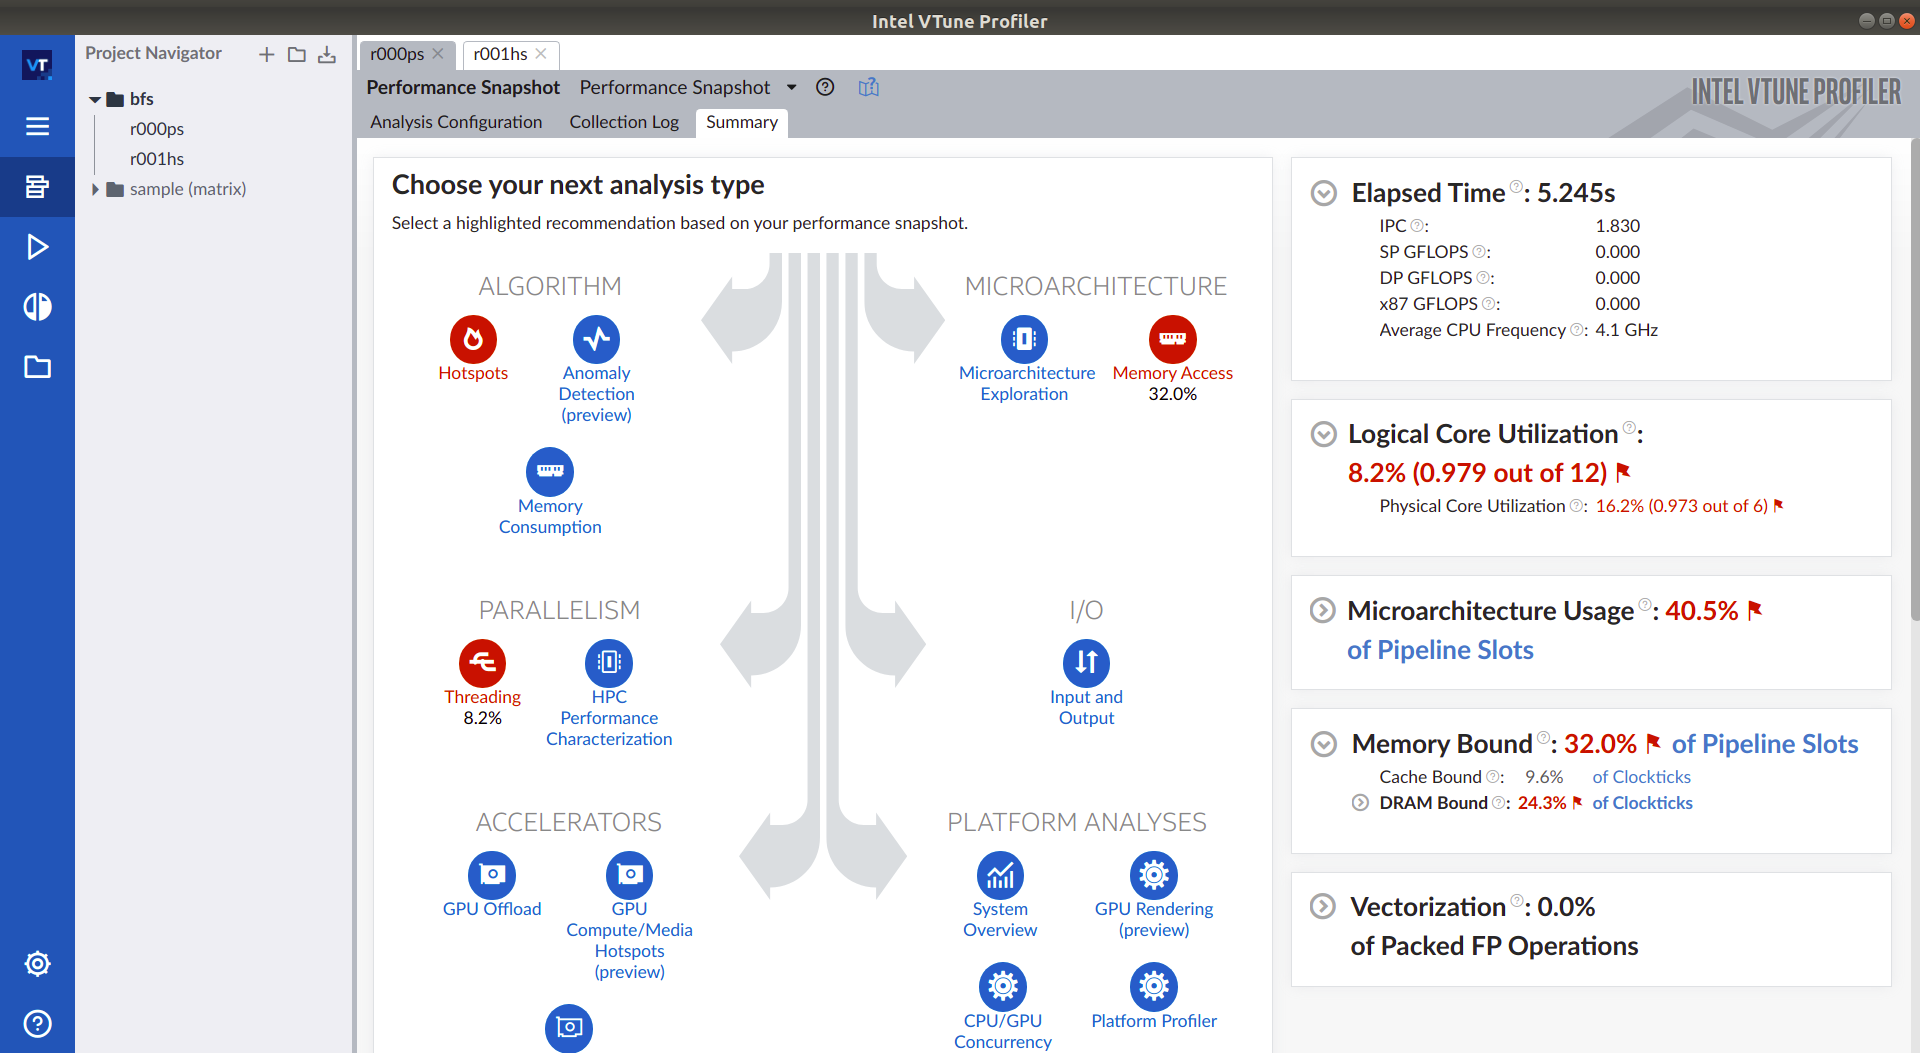
\includegraphics[scale=0.25]{vtune/bfs/ps.png}
    \caption{Performance Snapshot for \texttt{bfs.cpp}}
\end{figure}

\newpage
\subsection*{Top 5 Functions by CPU Time}
\begin{table}[H]
    \begin{tabular}{||l|l||c||}
        \hline
        Function                                                                      & Module                & CPU Time \\
        \hline
        \texttt{bfs}                                                                  & \texttt{bfs.o}        & 2.621s   \\
        \texttt{main}                                                                 & \texttt{bfs.o}        & 1.156s   \\
        \texttt{\_int\_free}                                                          & \texttt{libc-2.27.so} & 0.236s   \\
        \texttt{\_int\_malloc}                                                        & \texttt{libc-2.27.so} & 0.154s   \\
        \texttt{\_\_gnu\_cxx::new\_allocator<Node*>::construct<Node*, Node* const\&>} & \texttt{bfs.o}        & 0.124s   \\
        \hline
    \end{tabular}
\end{table}

\begin{figure}[H]
    \centering
    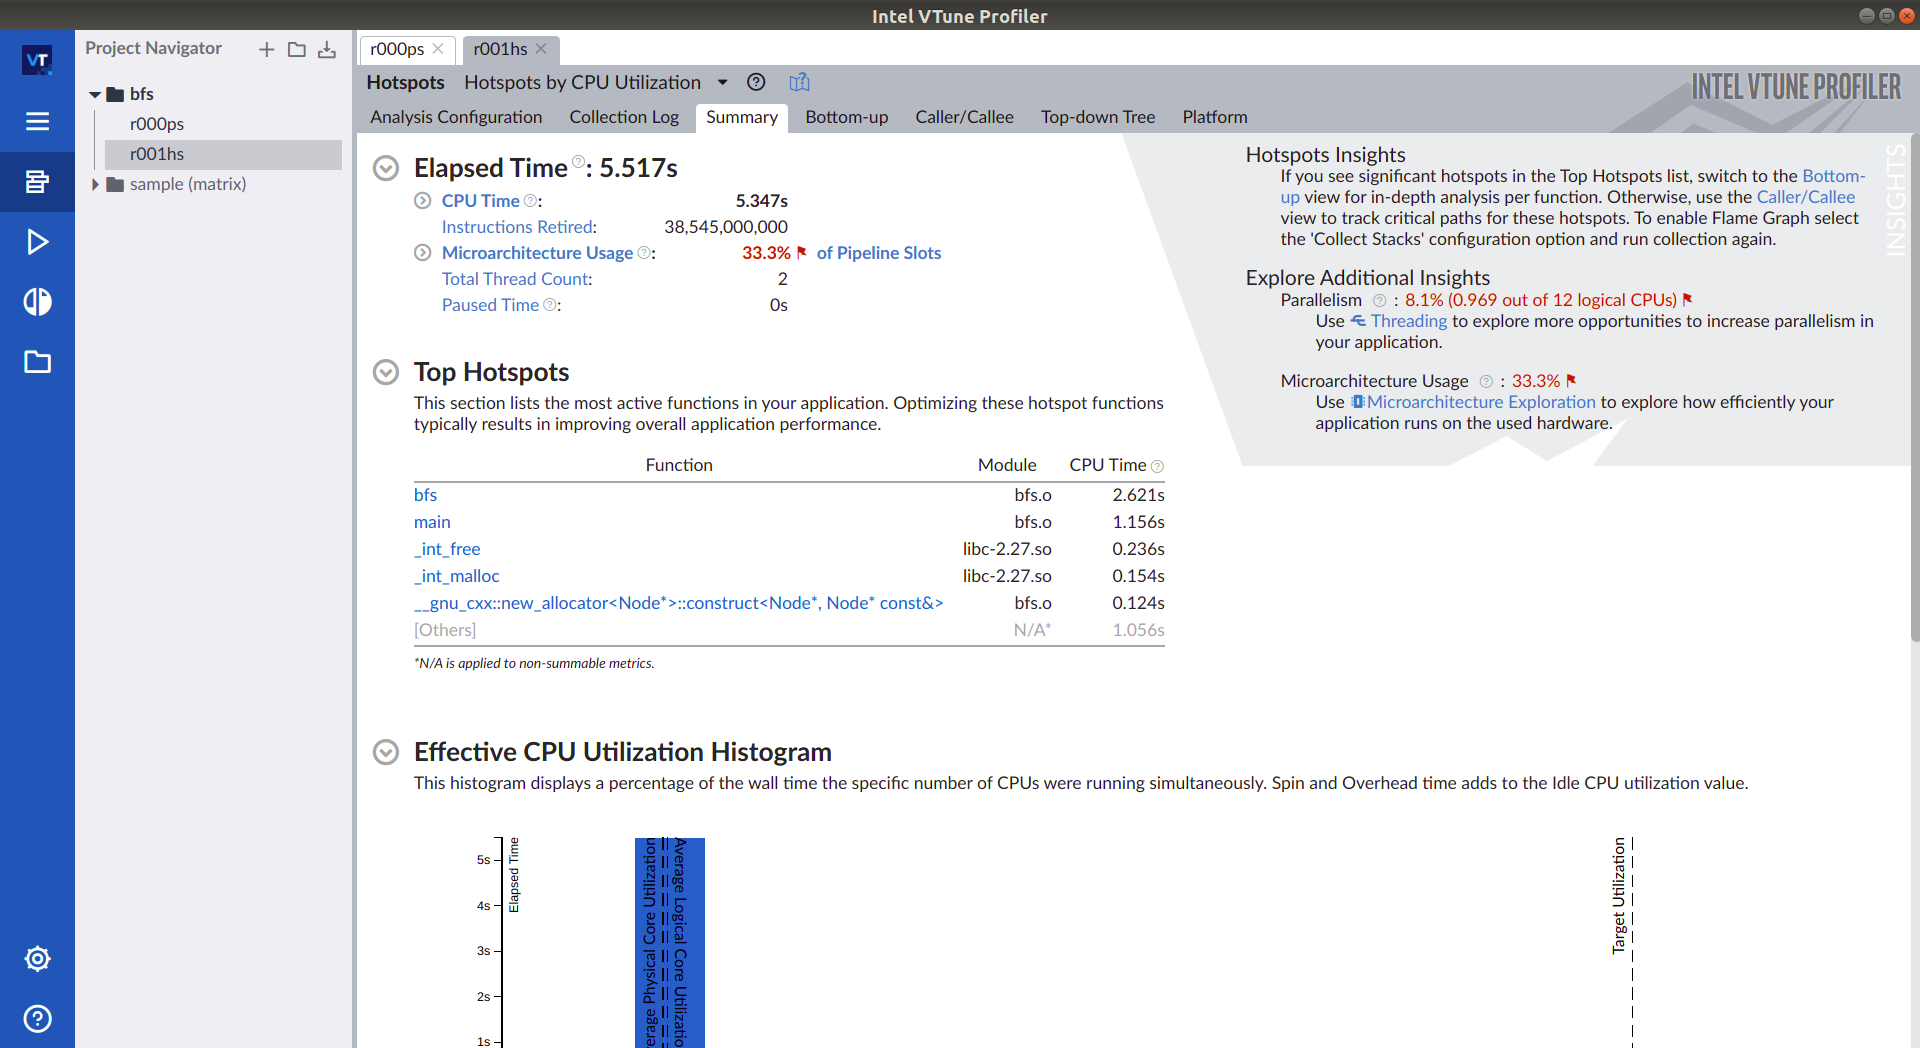
\includegraphics[scale=0.25]{vtune/bfs/hs.png}
    \caption{Top Functions by CPU Time for \texttt{bfs.cpp}}
\end{figure}

\newpage
\subsection*{Top 5 Source lines by CPU Utilization}
\begin{table}[H]
    \begin{tabular}{||l|l||c||}
        \hline
        Source                                               & Function                             & CPU Utilization \\
        \hline
        \texttt{if (left\_child) node\_Q.push(left\_child);} & \texttt{inline void bfs(Node *root)} & 22.7\%          \\
        \texttt{bfs(root);}                                  & \texttt{int main()}                  & 21.6\%          \\
        \texttt{right\_child = curr\_node->right;}           & \texttt{inline void bfs(Node *root)} & 17.2\%          \\
        \texttt{for (int i = 0; i < q\_size; i++) \{}        & \texttt{inline void bfs(Node *root)} & 4.8\%           \\
        \texttt{left\_child = curr\_node->left;}             & \texttt{inline void bfs(Node *root)} & 3.2\%           \\
        \hline
    \end{tabular}
\end{table}

\begin{figure}[H]
    \centering
    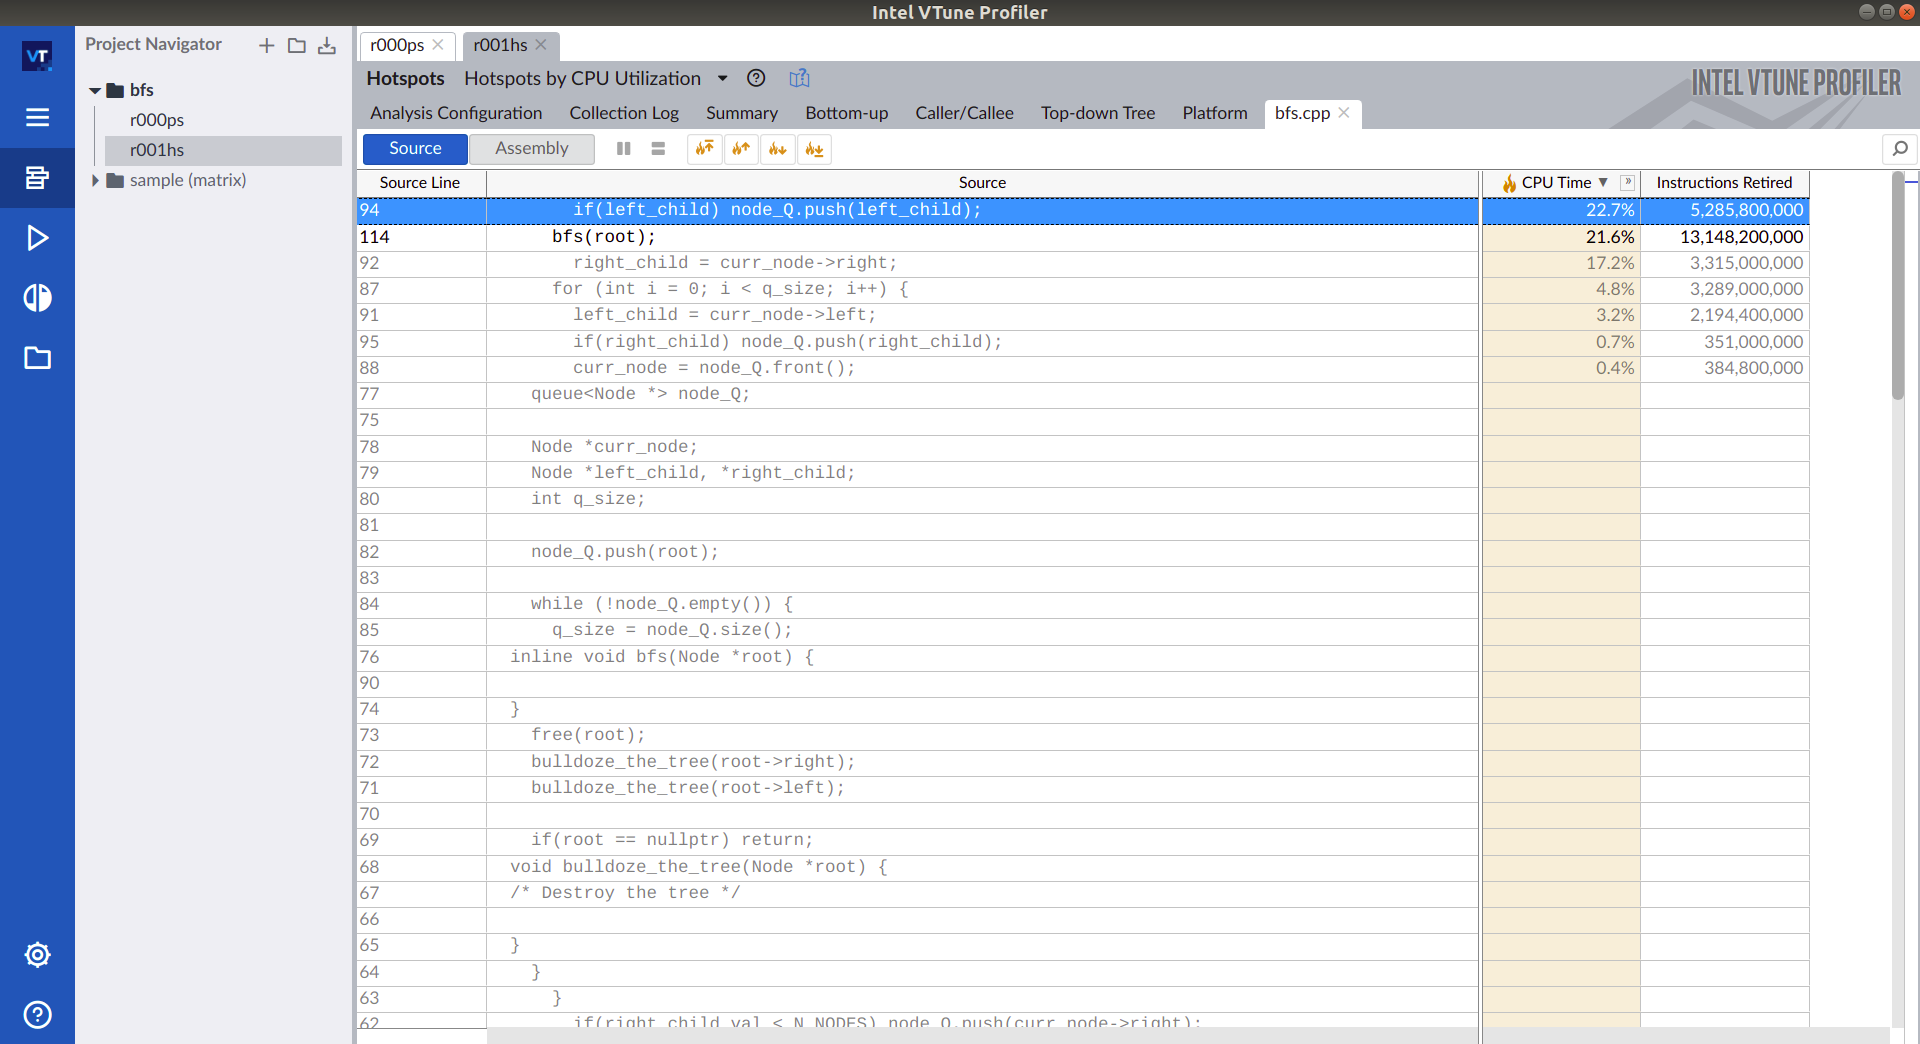
\includegraphics[scale=0.25]{vtune/bfs/sc.png}
    \caption{Top Source lines by CPU Utilization for \texttt{bfs.cpp}}
\end{figure}

\newpage
\section{\texttt{matrix\_multi.cpp}}

\subsection*{Performance Snapshot}
\begin{itemize}
    \item IPC: 0.874
    \item Logical Core Utilization: 8.2\% (0.982 out of 12)
    \item Physical Core Utilization: 16.3\% (0.976 of 6)
    \item Memory bound: 59.1\% of Pipeline slots
\end{itemize}

\begin{figure}[H]
    \centering
    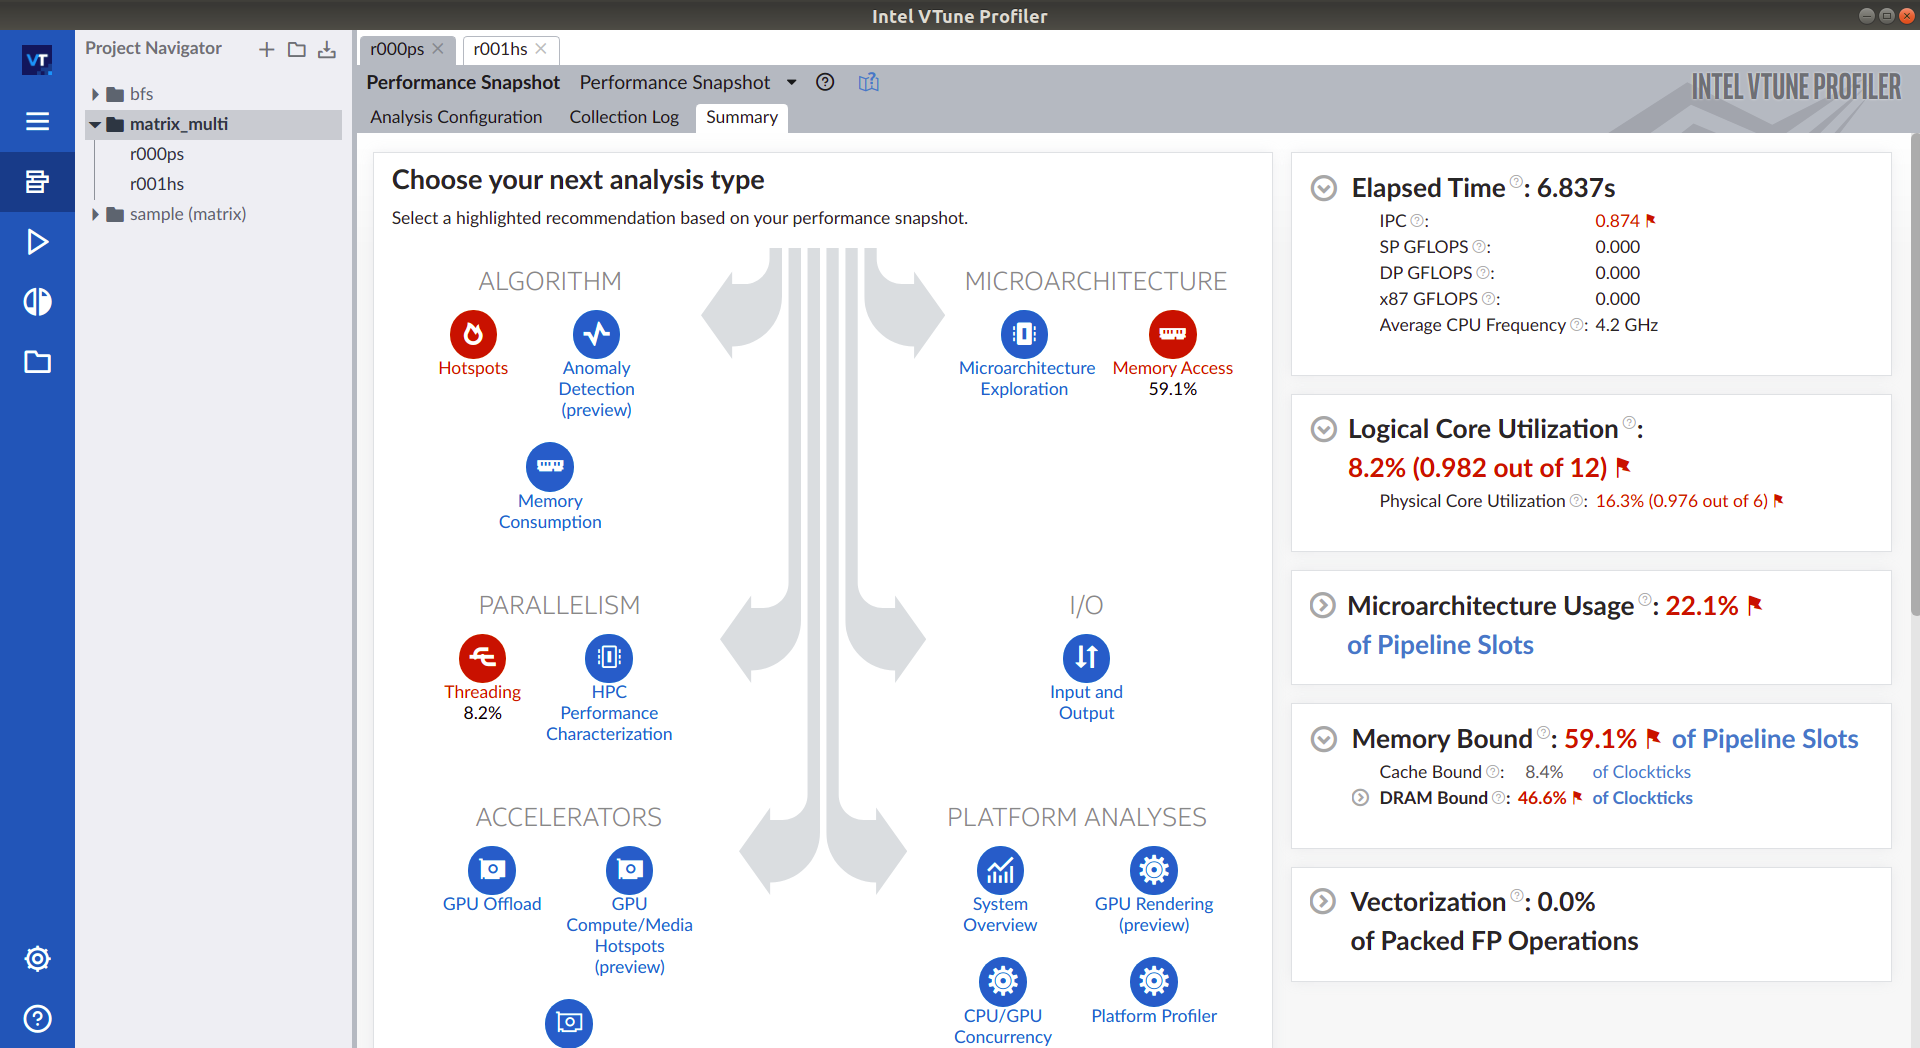
\includegraphics[scale=0.25]{vtune/matrix_multi/ps.png}
    \caption{Performance Snapshot for \texttt{matrix\_multi.cpp}}
\end{figure}

\newpage
\subsection*{Top Functions by CPU Time}
\begin{table}[H]
    \begin{tabular}{||l|l||c||}
        \hline
        Function                 & Module                   & CPU Time \\
        \hline
        \texttt{matrix\_product} & \texttt{matrix\_multi.o} & 6.597s   \\
        \hline
    \end{tabular}
\end{table}

\begin{figure}[H]
    \centering
    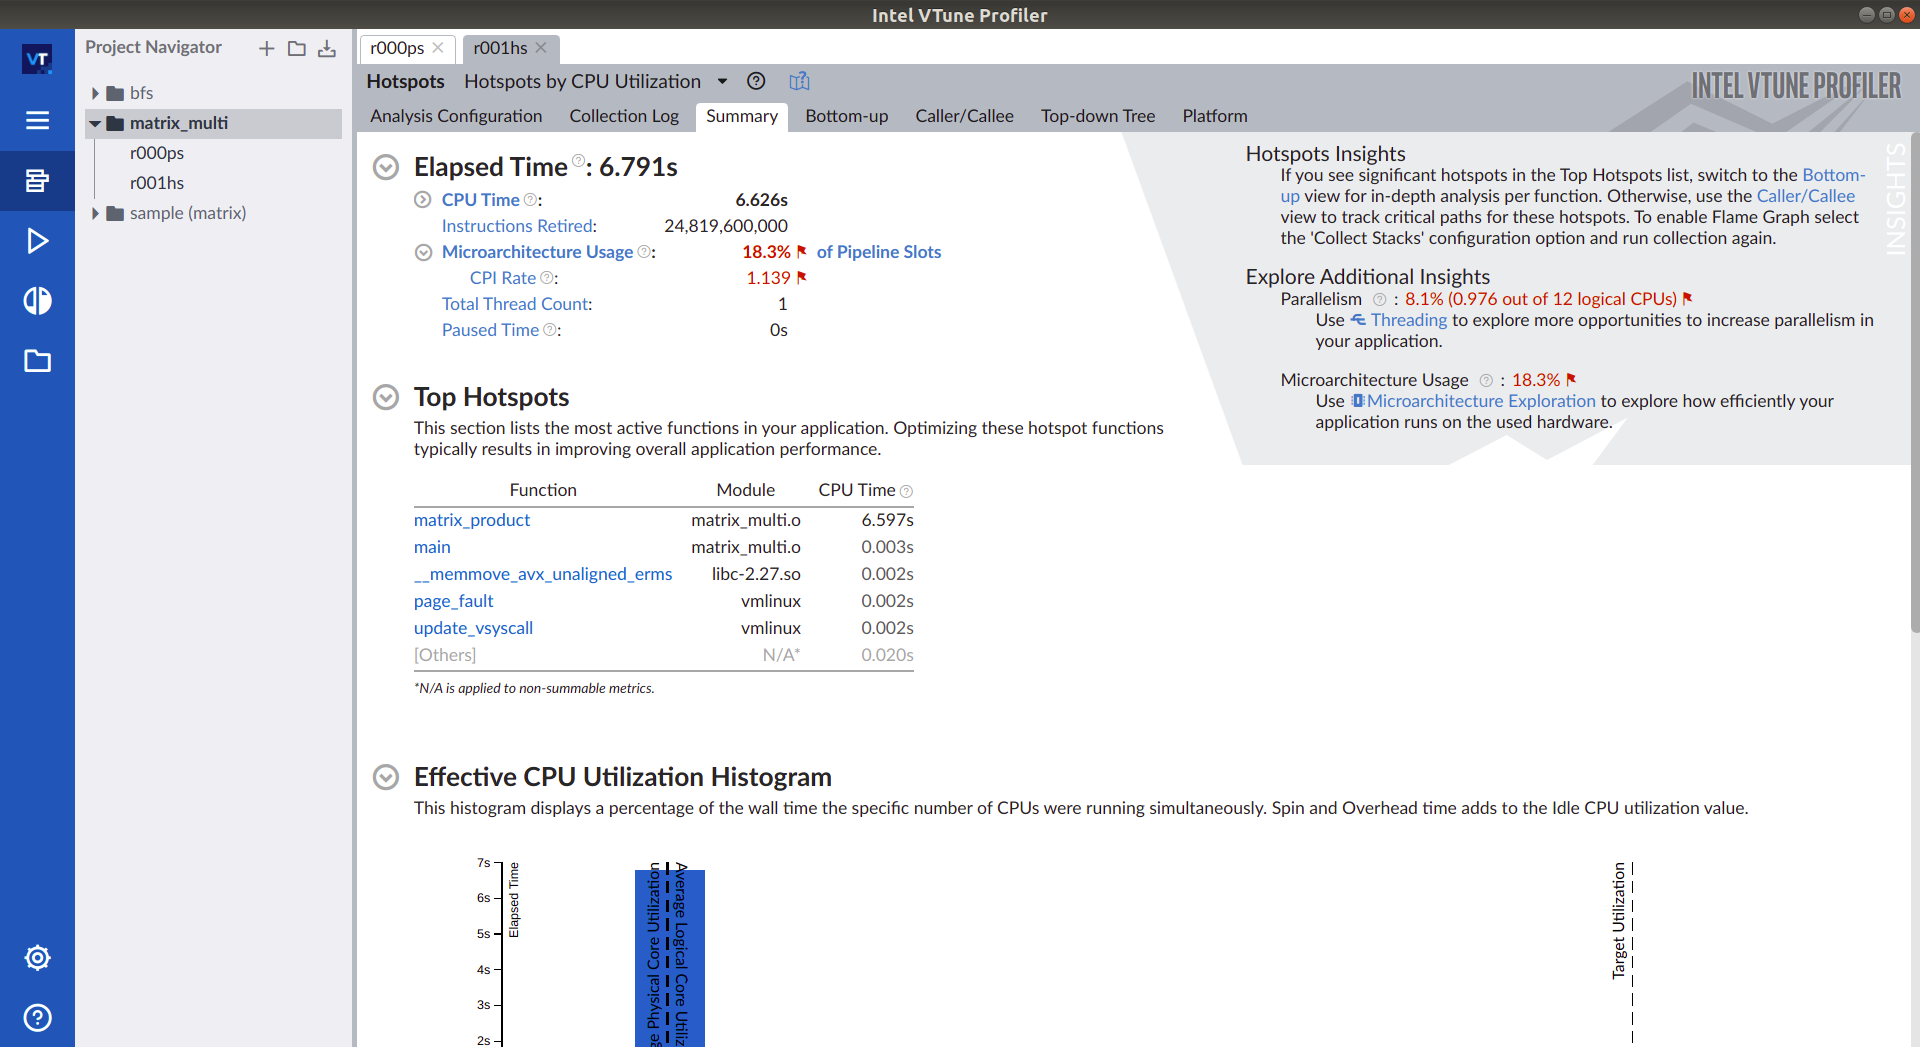
\includegraphics[scale=0.25]{vtune/matrix_multi/hs.png}
    \caption{Top Functions by CPU Time for \texttt{matrix\_multi.cpp}}
\end{figure}

\newpage
\subsection*{Top 2 Source lines by CPU Utilization}
\begin{table}[H]
    \begin{tabular}{||l|l||c||}
        \hline
        Source                                        & Function                        & CPU Utilization \\
        \hline
        \texttt{C[i][j] += A[i][k] * B[k][j];}        & \texttt{void matrix\_product()} & 90.9\%          \\
        \texttt{for (int k = 0; k < N\_DIMS; k++) \{} & \texttt{void matrix\_product()} & 8.6\%           \\
        \hline
    \end{tabular}
\end{table}

\begin{figure}[H]
    \centering
    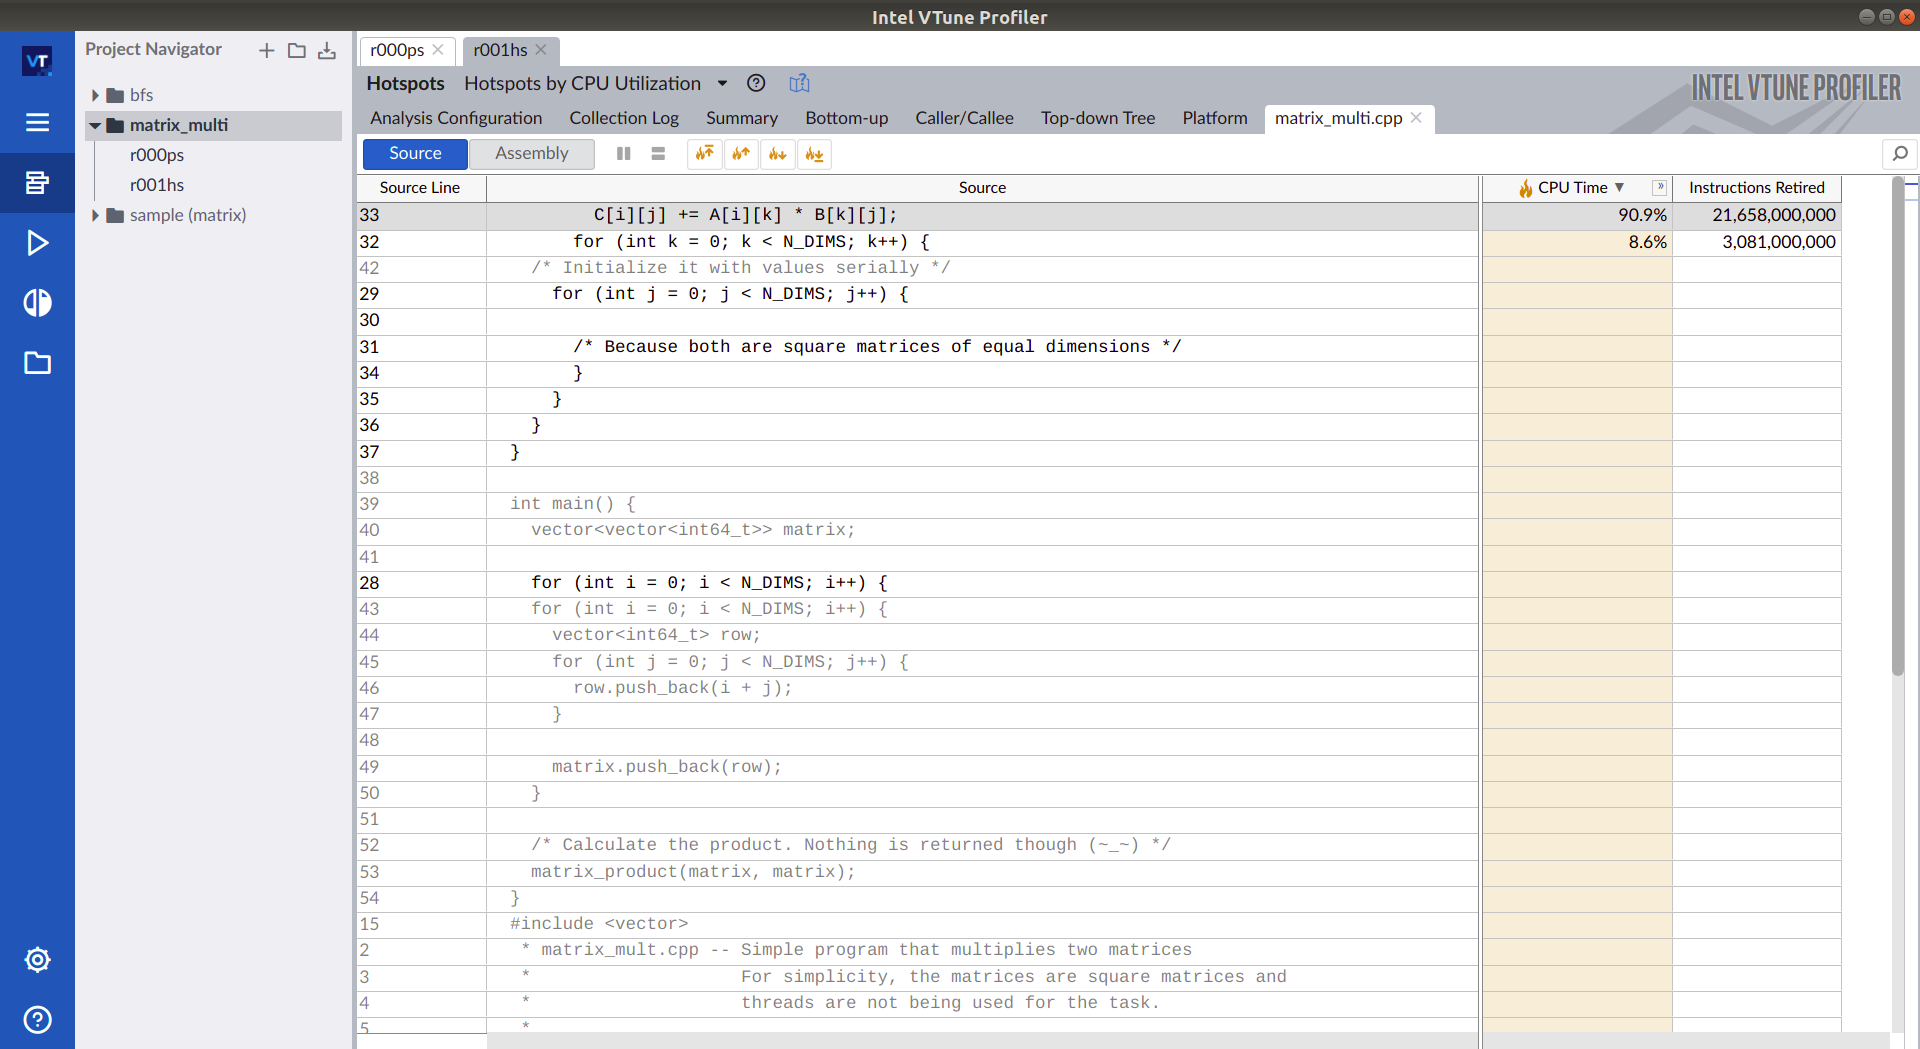
\includegraphics[scale=0.25]{vtune/matrix_multi/sc.png}
    \caption{Top Source lines by CPU Utilization for \texttt{matrix\_multi.cpp}}
\end{figure}

\newpage
\section{\texttt{matrix\_multi\_2.cpp}}

\subsection*{Performance Snapshot}
\begin{itemize}
    \item IPC: 1.339
    \item Logical Core Utilization: 8.2\% (0.981 out of 12)
    \item Physical Core Utilization: 16.2\% (0.973 of 6)
    \item Memory bound: 38.0\% of Pipeline slots
\end{itemize}

\begin{figure}[H]
    \centering
    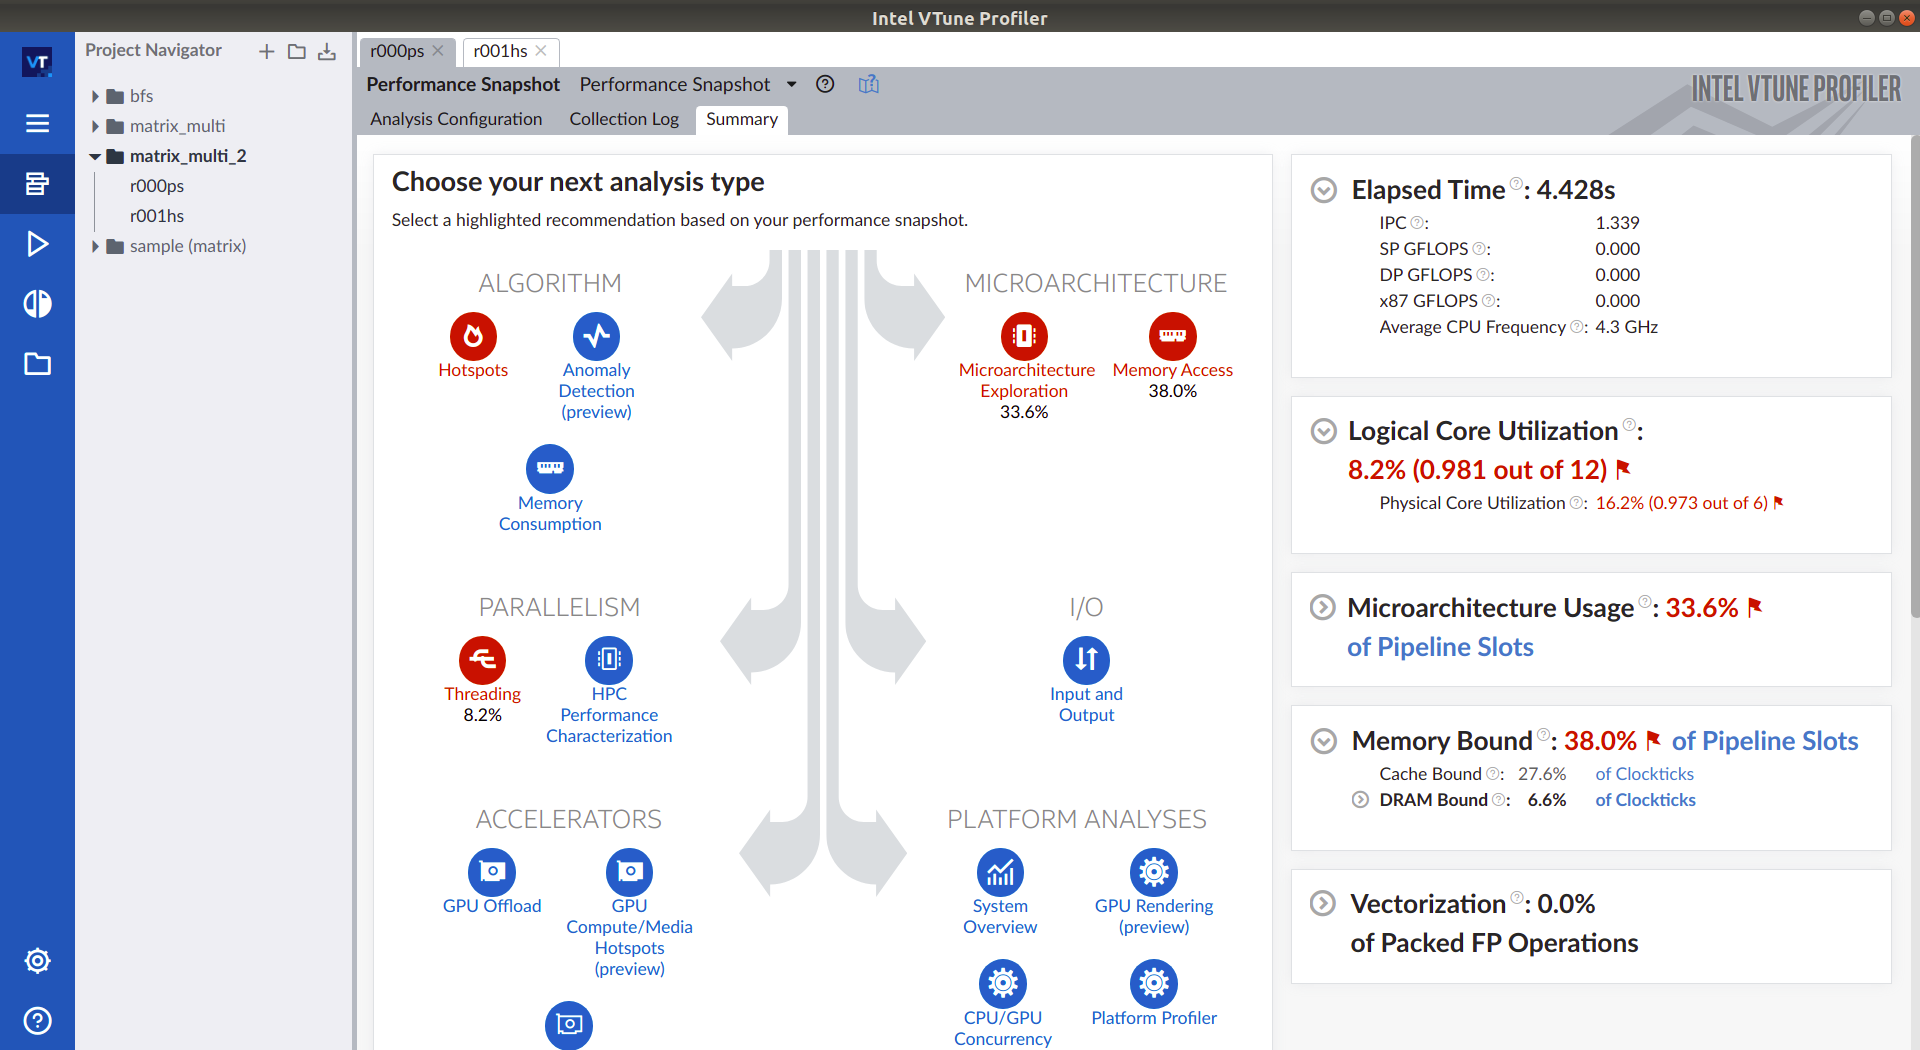
\includegraphics[scale=0.25]{vtune/matrix_multi_2/ps.png}
    \caption{Performance Snapshot for \texttt{matrix\_multi\_2.cpp}}
\end{figure}

\newpage
\subsection*{Top Functions by CPU Time}
\begin{table}[H]
    \begin{tabular}{||l|l||c||}
        \hline
        Function                 & Module                      & CPU Time \\
        \hline
        \texttt{matrix\_product} & \texttt{matrix\_multi\_2.o} & 4.492s   \\
        \hline
    \end{tabular}
\end{table}

\begin{figure}[H]
    \centering
    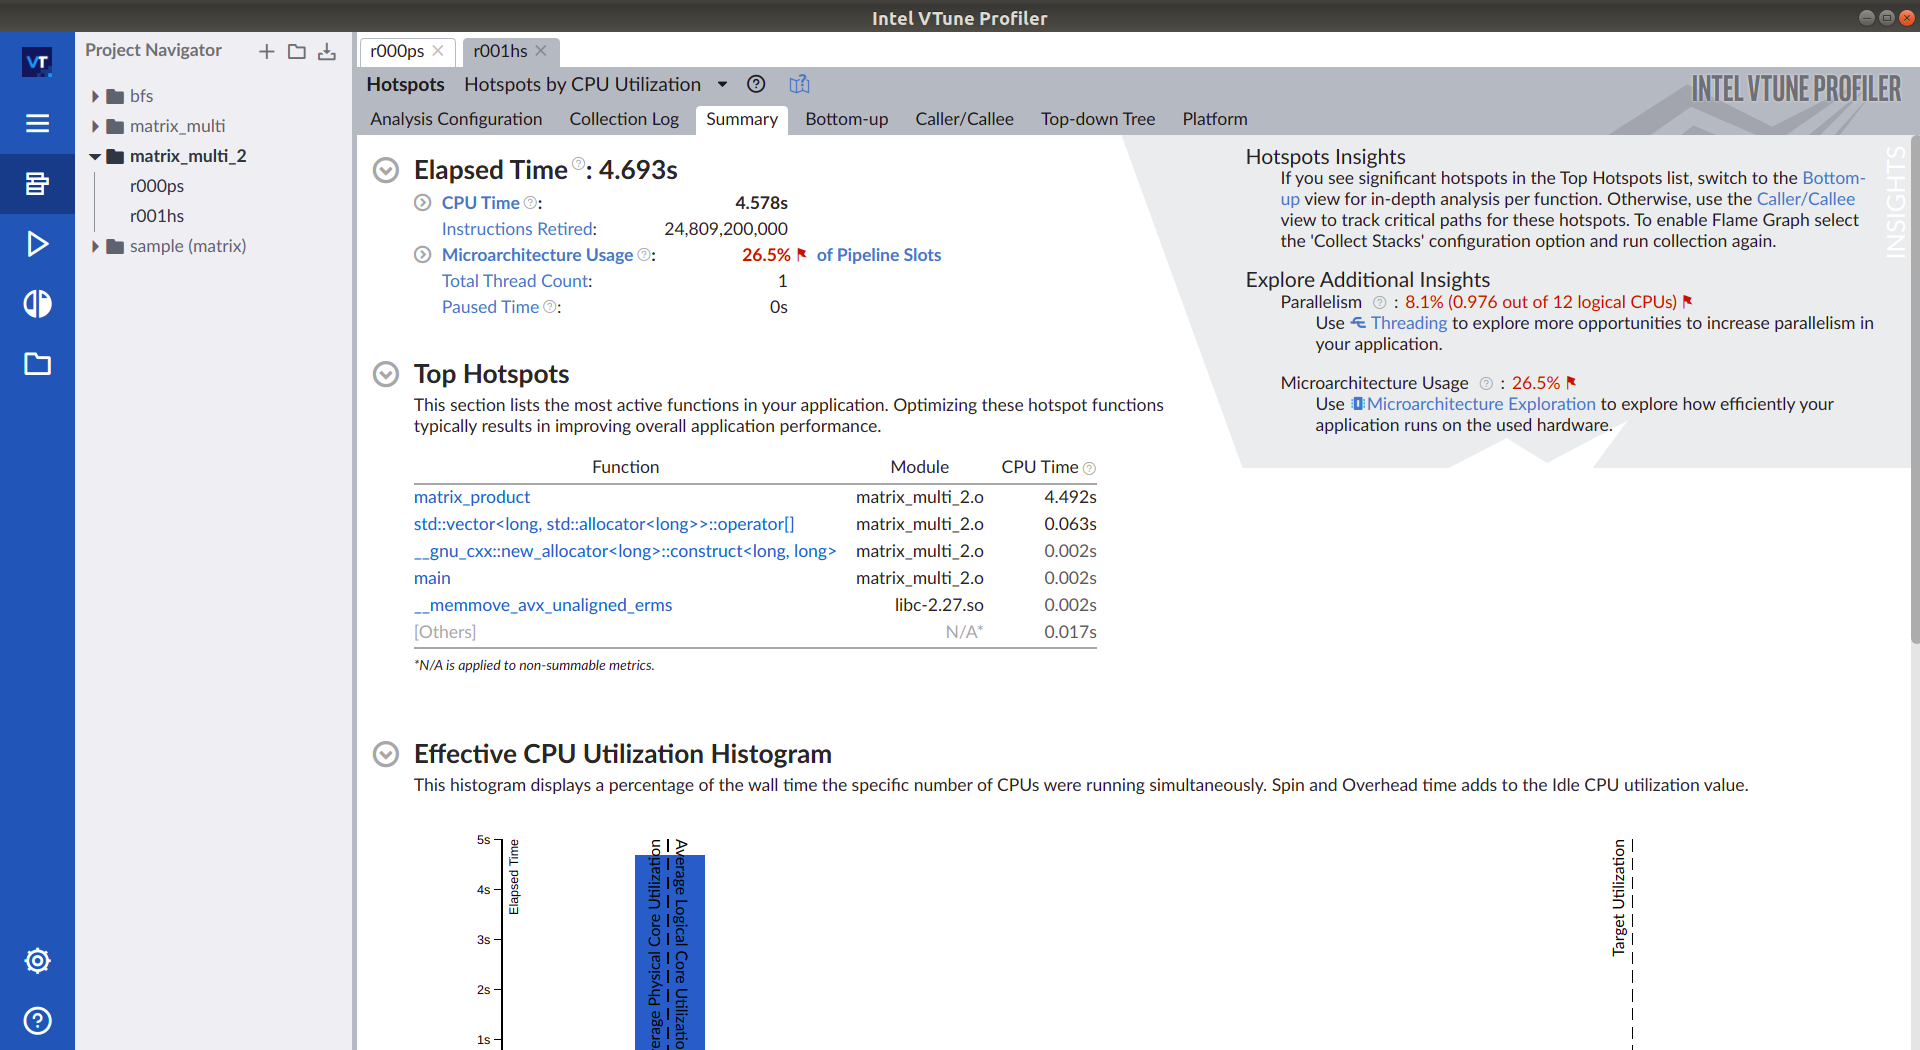
\includegraphics[scale=0.25]{vtune/matrix_multi_2/hs.png}
    \caption{Top Functions by CPU Time for \texttt{matrix\_multi\_2.cpp}}
\end{figure}

\newpage
\subsection*{Top 2 Source lines by CPU Utilization}
\begin{table}[H]
    \begin{tabular}{||l|l||c||}
        \hline
        Source                                        & Function                        & CPU Utilization \\
        \hline
        \texttt{C[i][j] += A[i][k] * B[k][j];}        & \texttt{void matrix\_product()} & 84.4\%          \\
        \texttt{for (int k = 0; k < N\_DIMS; k++) \{} & \texttt{void matrix\_product()} & 13.7\%          \\
        \hline
    \end{tabular}
\end{table}

\begin{figure}[H]
    \centering
    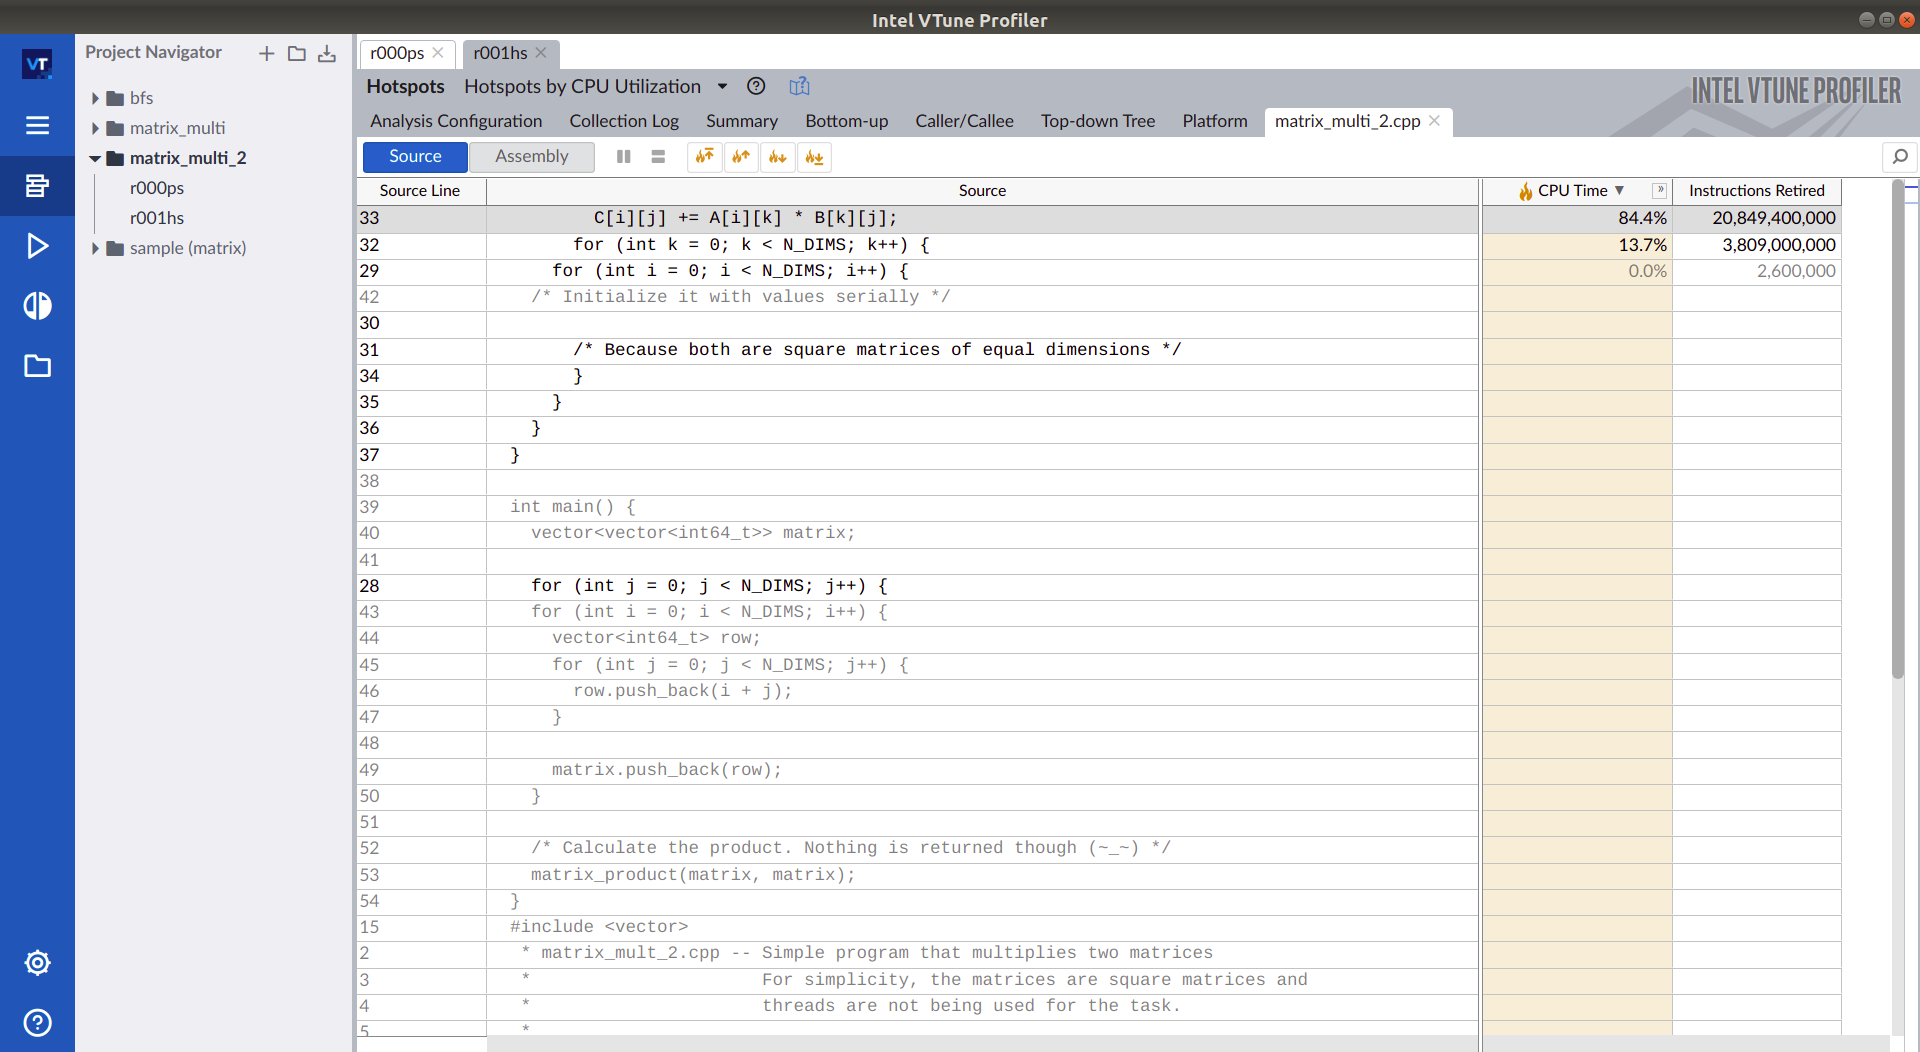
\includegraphics[scale=0.25]{vtune/matrix_multi_2/sc.png}
    \caption{Top Source lines by CPU Utilization for \texttt{matrix\_multi\_2.cpp}}
\end{figure}

\newpage
\section{\texttt{quicksort.cpp}}

\subsection*{Performance Snapshot}
\begin{itemize}
    \item IPC: 0.748
    \item Logical Core Utilization: 8.0\% (0.966 out of 12)
    \item Physical Core Utilization: 15.7\% (0.941 of 6)
    \item Memory bound: 23.0\% of Pipeline slots
\end{itemize}

\begin{figure}[H]
    \centering
    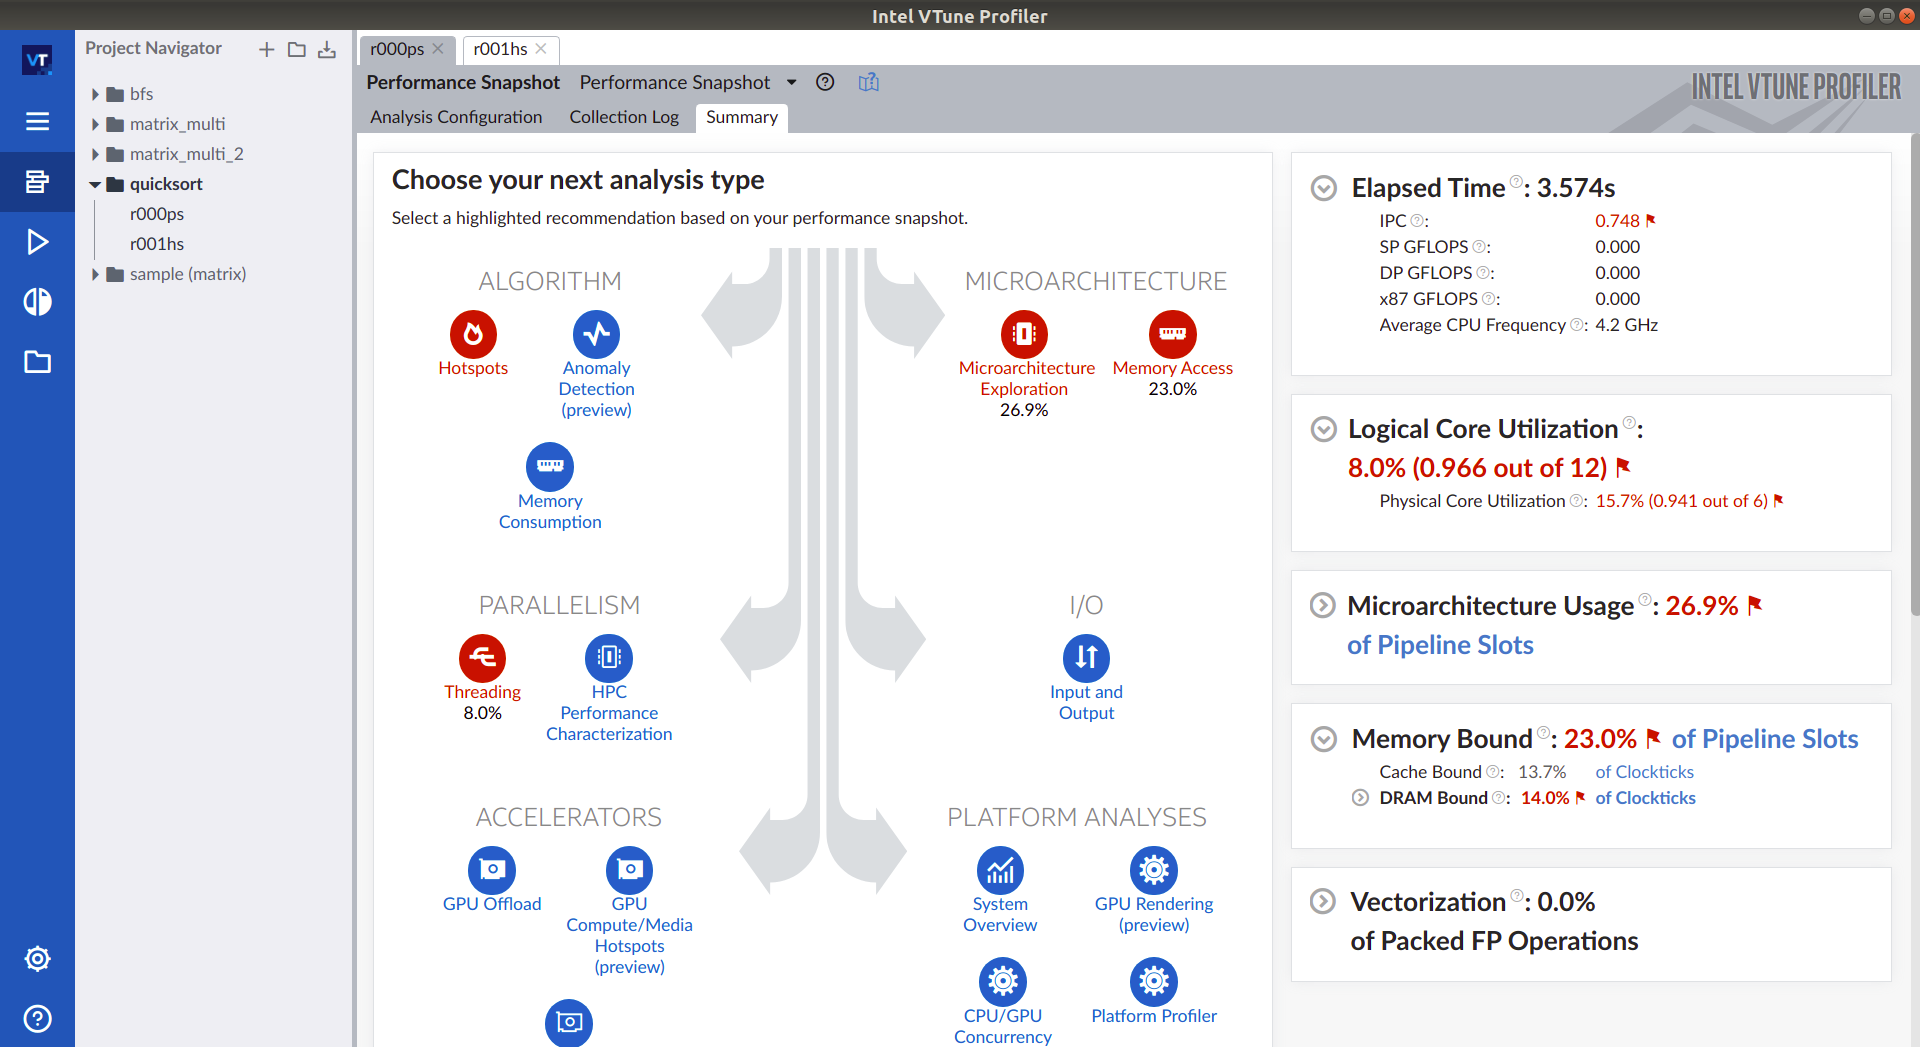
\includegraphics[scale=0.25]{vtune/quicksort/ps.png}
    \caption{Performance Snapshot for \texttt{quicksort.cpp}}
\end{figure}

\newpage
\subsection*{Top Functions by CPU Time}
\begin{table}[H]
    \begin{tabular}{||l|l||c||}
        \hline
        Function                                   & Module                & CPU Time \\
        \hline
        \texttt{\_\_memmove\_avx\_unaligned\_erms} & \texttt{libc-2.27.so} & 0.875s   \\
        \texttt{page\_fault}                       & \texttt{vmlinux}      & 0.511s   \\
        \texttt{clear\_page\_erms}                 & \texttt{vmlinux}      & 0.228s   \\
        \texttt{prepare\_exit\_to\_usermode}       & \texttt{vmlinux}      & 0.226s   \\
        \texttt{perf\_iterate\_ctx}                & \texttt{vmlinux}      & 0.155s   \\
        Others                                     & N/A                   & 1.545s   \\
        \hline
    \end{tabular}
\end{table}

\begin{figure}[H]
    \centering
    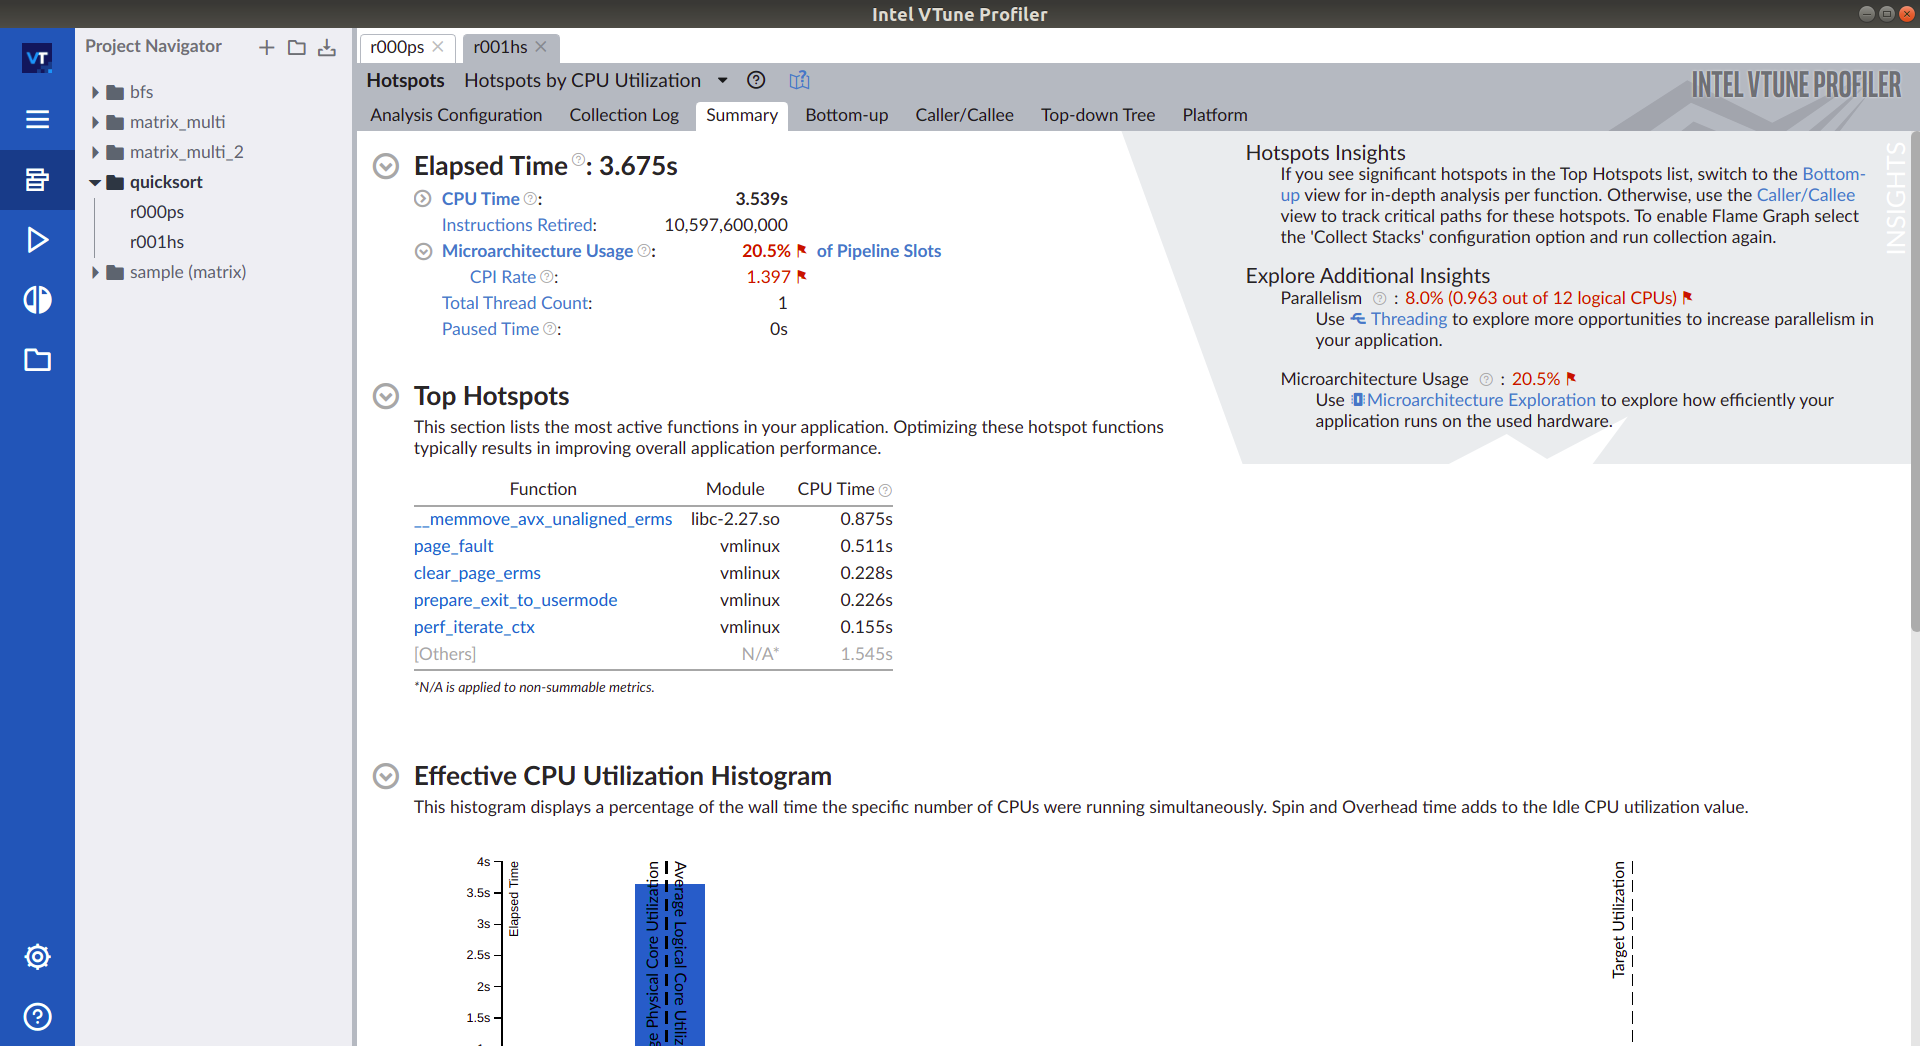
\includegraphics[scale=0.25]{vtune/quicksort/hs.png}
    \caption{Top Functions by CPU Time for \texttt{quicksort.cpp}}
\end{figure}

\newpage
\subsection*{Top 5 Source lines by CPU Utilization}
\begin{table}[H]
    \begin{tabular}{||l|l||c||}
        \hline
        Source                                     & Function                  & CPU Utilization \\
        \hline
        \texttt{b = c;}                            & \texttt{void swap()}      & 2.1\%           \\
        \texttt{if (nums[i] < pivot) \{}           & \texttt{long partition()} & 1.9\%           \\
        \texttt{slow\_ptr++;}                      & \texttt{long partition()} & 1.7\%           \\
        \texttt{for (long i = lo; i < hi; i++) \{} & \texttt{long partition()} & 0.6\%           \\
        \texttt{a = b;}                            & \texttt{void swap()}      & 0.2\%           \\
        \hline
    \end{tabular}
\end{table}

\begin{figure}[H]
    \centering
    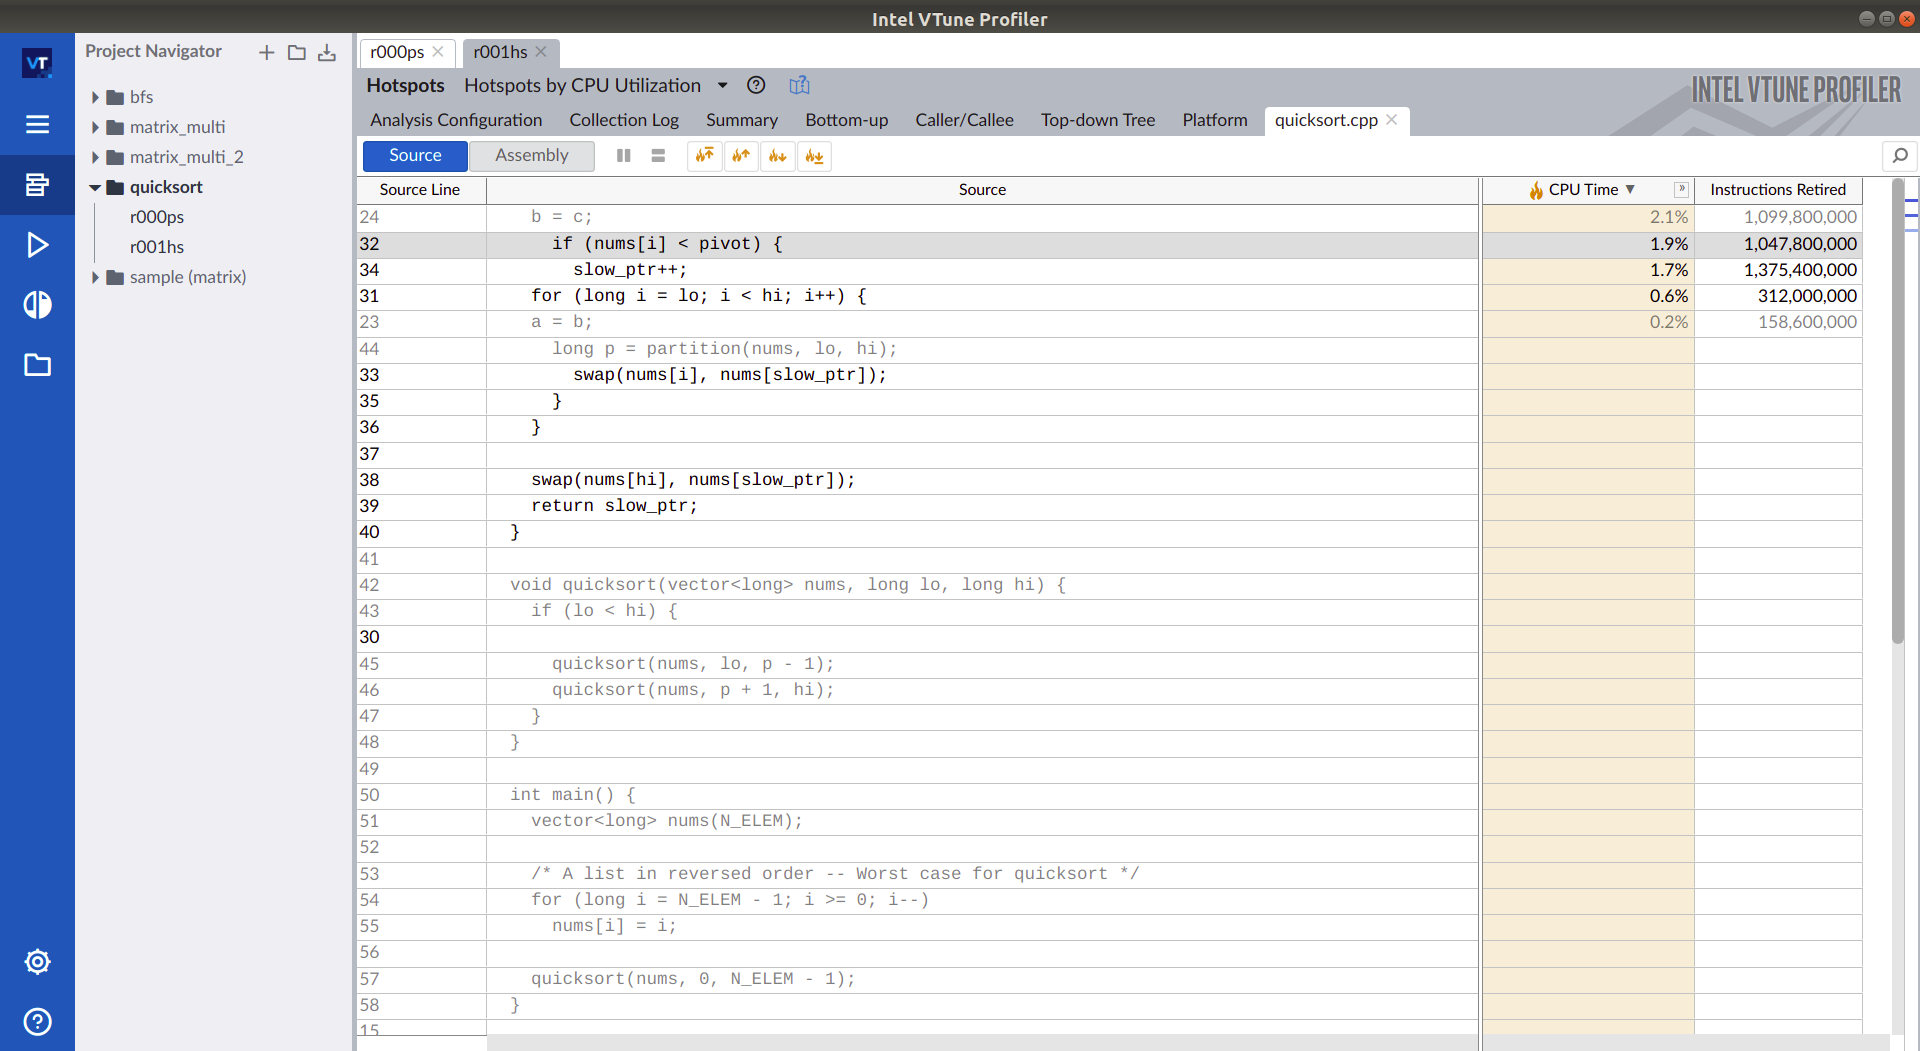
\includegraphics[scale=0.25]{vtune/quicksort/sc.png}
    \caption{Top Source lines by CPU Utilization for \texttt{quicksort.cpp}}
\end{figure}


%%%%%%%%%%%%%%%%%%%%%%%%%%%%%%%%%%%%%%%%%%%%%%%%
%% Part 2: Simulating with ChampSim
%%%%%%%%%%%%%%%%%%%%%%%%%%%%%%%%%%%%%%%%%%%%%%%%
\chapter{Simulating with ChampSim}
\section{Prepare traces}

Generate tracer for champsim: \\
\texttt{cd /champsim/ChampSim/tracer; ./make\_tracer.sh;} \\
Used pin to generate traces: \\
\texttt{pin -t obj-intel64/champsim\_tracer.so -o <program>.trace -t 21000000 -- <executable>;} \\
Used xz to compress the traces: \\
\texttt{xz -vz <program>.trace --threads=0;}

\begin{table}[H]
    \begin{tabular}{||l||l|c||c||}
        \hline
        Program                     & Parameters                                         & Execution time & Trace size \\
        \hline
        \texttt{bfs.o}              & \texttt{N\_NODES (1<<15)}; \texttt{N\_LOOPS 1000}; & 3.4 s          & 2092 KB    \\
        \hline
        \texttt{matrix\_multi.o}    & \texttt{N\_DIMS 700};                              & 4.5 s          & 2172 KB    \\
        \hline
        \texttt{matrix\_multi\_2.o} & \texttt{N\_DIMS 700};                              & 4.2 s          & 2160 KB    \\
        \hline
        \texttt{quicksort.o}        & \texttt{N\_ELEM (1<<14)};                          & 3.1 s          & 4172 KB    \\
        \hline
    \end{tabular}
\end{table}


\end{document}
